\documentclass[12pt]{article}
\usepackage{url,graphicx,tabularx,array,geometry,enumitem,amsmath}
\setlength{\parskip}{1ex} %--skip lines between paragraphs
\setlength{\parindent}{0pt} %--don't indent paragraphs

%-- Commands for header
\renewcommand{\title}[1]{\textbf{#1}\\}
\renewcommand{\line}{\begin{tabularx}{\textwidth}{X>{\raggedleft}X}\hline\\\end{tabularx}\\[-0.5cm]}
\newcommand{\leftright}[2]{\begin{tabularx}{\textwidth}{X>{\raggedleft}X}#1%
& #2\\\end{tabularx}\\[-0.5cm]}

%\linespread{2} %-- Uncomment for Double Space
\begin{document}

\title{Digital Signal Processing - Assignment 5}
\line
\leftright{\today}{Stephanie Lund (2555914)\\Aljoscha Dietrich (2557976)} %-- left and right positions in the header

\section*{Exercise 1}

\subsection*{1.1}
See included file $'hw5.m'$.

\subsection*{1.2}
TODO: finish code and generate graph
% 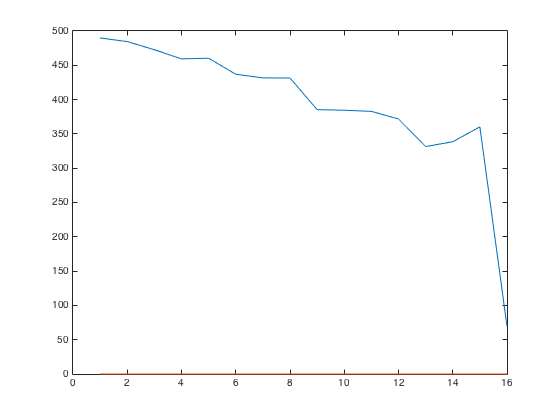
\includegraphics[scale=0.5]{hw5-1.png}

\section*{Exercise 2}
TODO

\section*{Bonus}
TODO

\end{document}